%
%%%%%%%%%%%%%%%%%%%%%%%%%%%%%%%%%%%%%%%%%%%%%%%%%%%%%%%%%%%%%%%%%%%%%%%%
\chapter{GitLab Issues}
%%%%%%%%%%%%%%%%%%%%%%%%%%%%%%%%%%%%%%%%%%%%%%%%%%%%%%%%%%%%%%%%%%%%%%%%
%
GitLab Issues is the bug/development tracker of the \telemacsystem. It is
available at the following address:\\
\url{https://gitlab.pam-retd.fr/otm/telemac-mascaret/-/issues}.
In order to login, you need to use your GitLab login and password.
%
%
\section{Creating an issue}
%
%
To create a new issue, you must click on ``New issue''. This will lead you to
the page shown on Fig \ref{fig:gitlab-issue}. You will then need to fill the
following information:
\begin{itemize}
\item Title: title of the issue.
\item Type: Issue or Incident (this field should usually remain on ``Issue'').
\item Description: give a full explication of the problem.
\item Assignee: person in charge of the development integration.
\item Due date: deadline to ensure that the fix or feature is integrated on
  time.
\item Milestone: target version of the code in which the development should be
  integrated.
\item Labels: tags related to the type of the issue (bug, feature or
enhancement), the module which is concerned, the area of the system...
\end{itemize}
\begin{figure}[H]
    \centering
    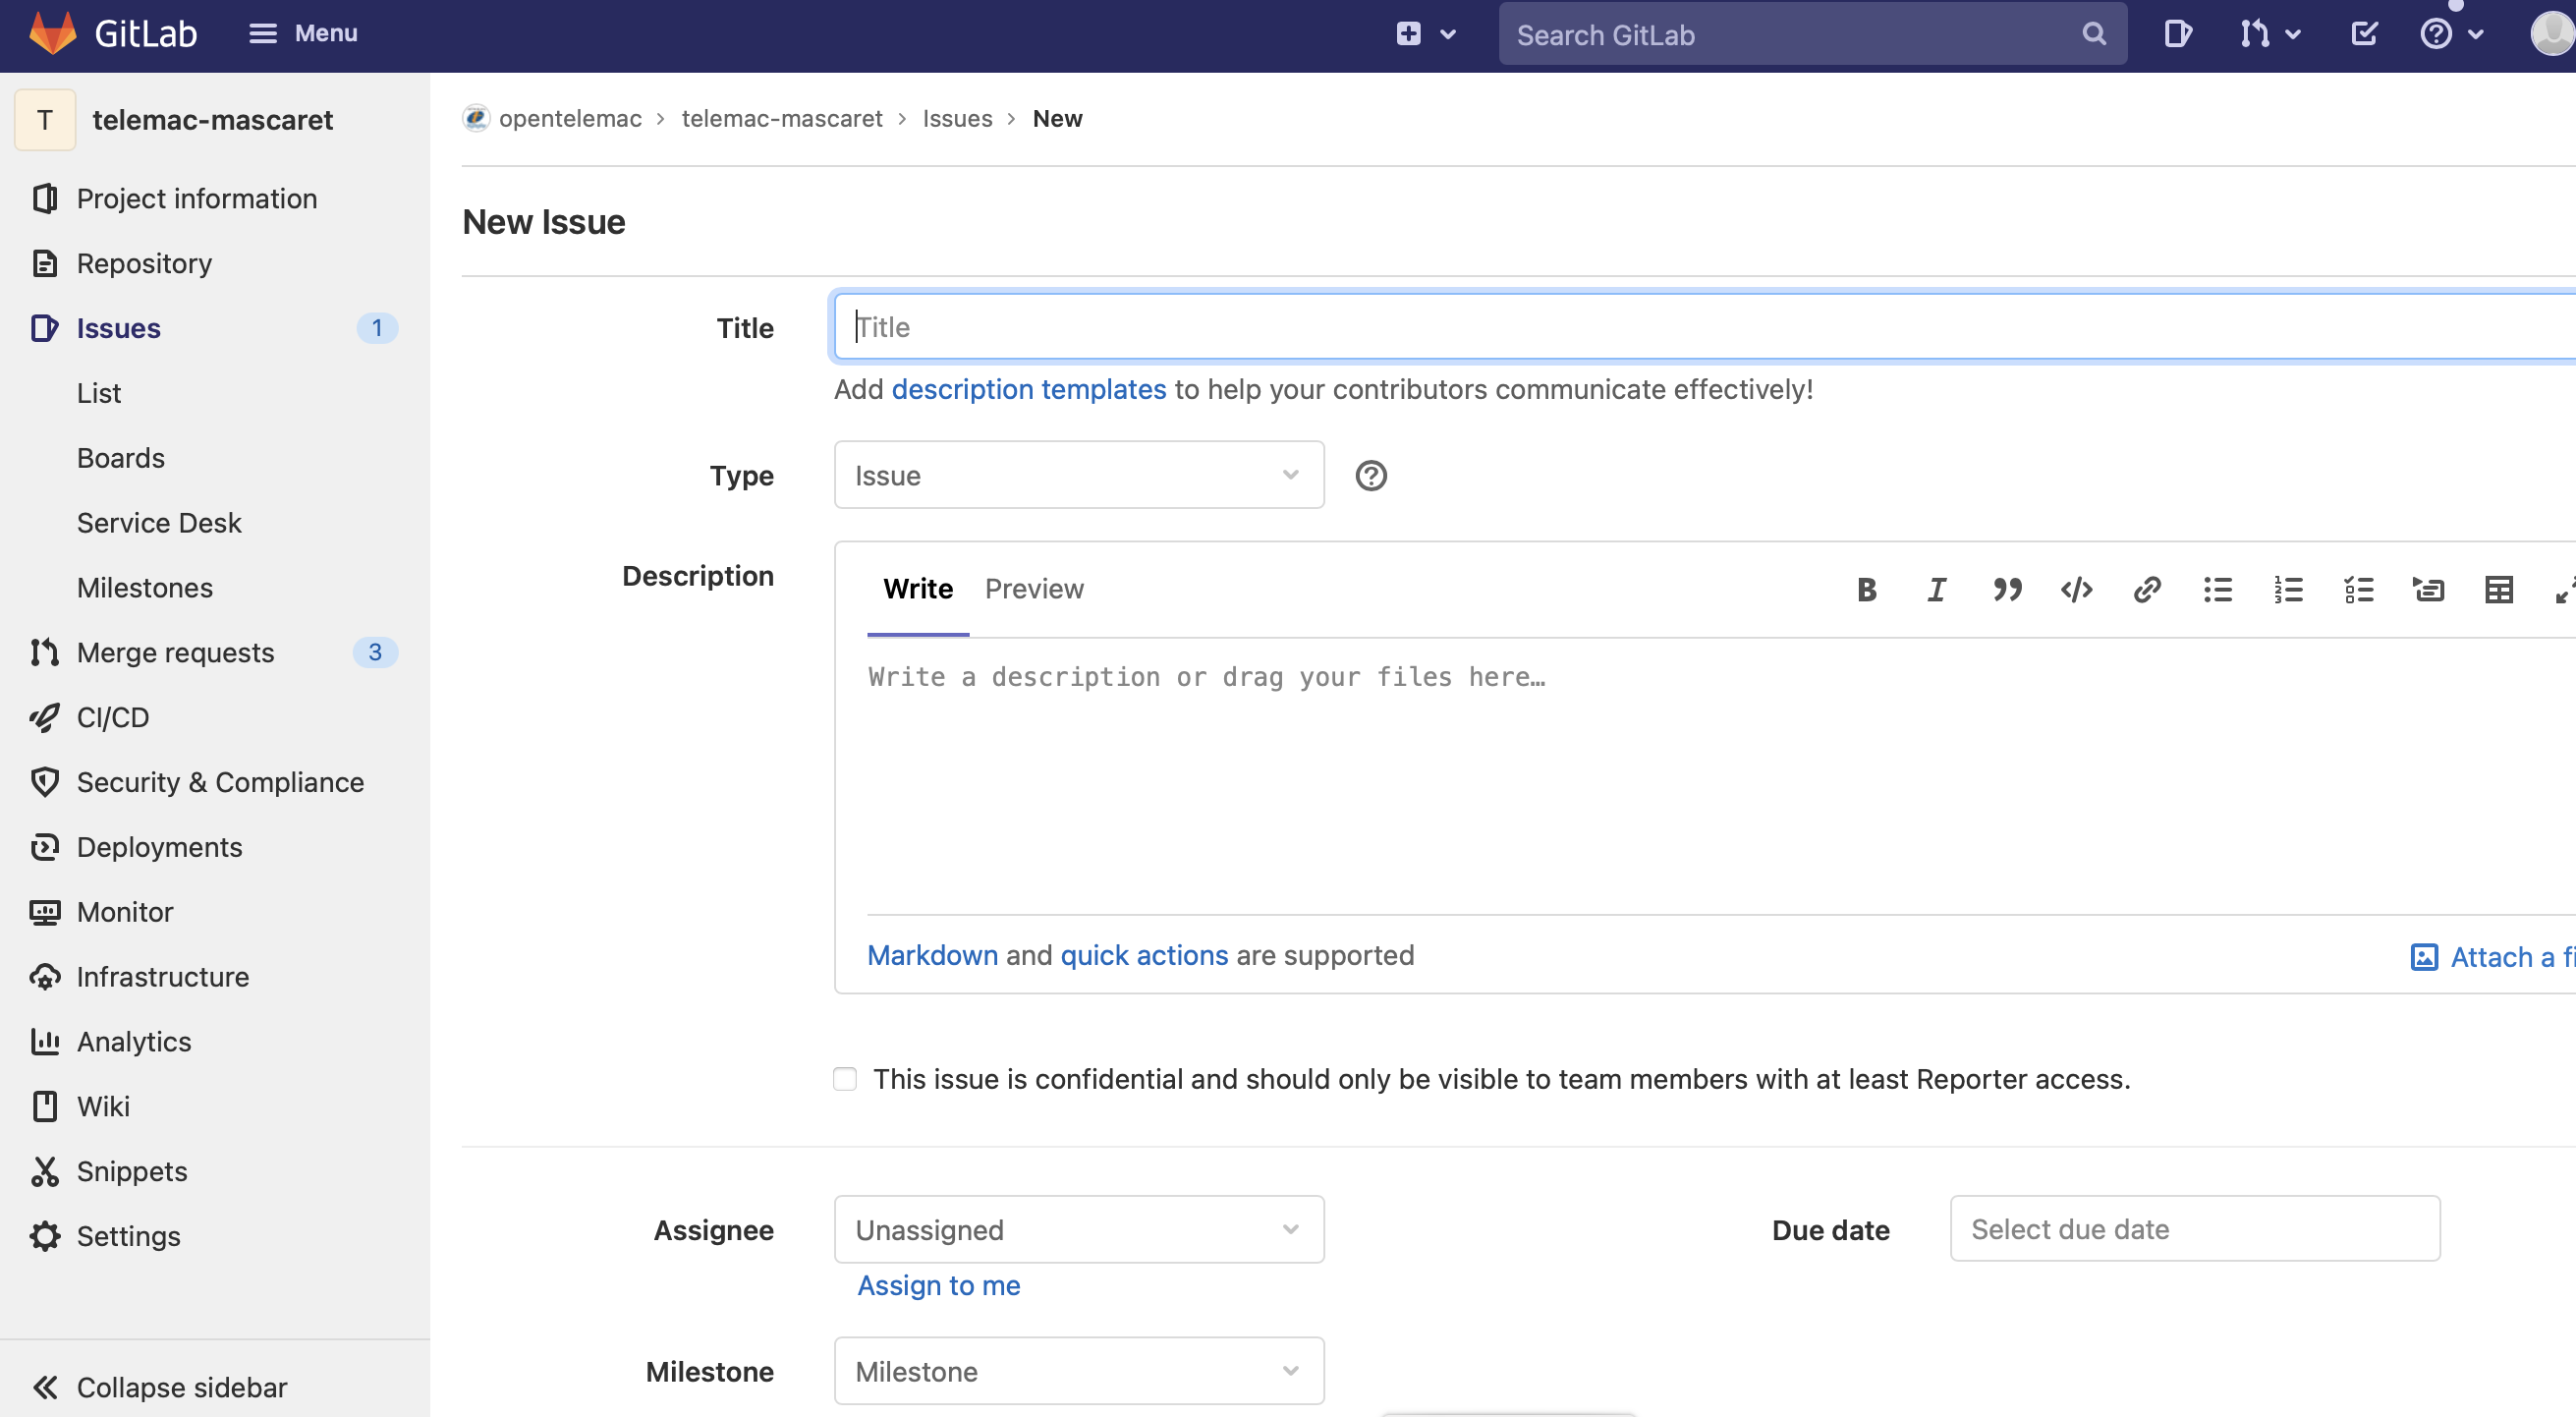
\includegraphics[scale=0.3]{graphics/issue-creation.png}
    \caption{Creation of an issue}
    \label{fig:gitlab-issue}
\end{figure}
%
%
\section{Modifying an issue}
%
%
To change an issue content (title, description...), go to the issue and then
click on ``Edit Issue''. The Fig \ref{fig:gitlab-issue} shows the page that is
displayed when clicking on an issue.

You will have to update your issue as your work advances, either by adding
comments on what you have done or by changing its status. For example, when a
bug has been resolved, you can close the issue by clicking on ``Close Issue''
once the correction has been integrated into the main branch.
%
